\section{Design of UP-SSO}
\label{sec:design}
\begin{figure*}[t!]
  \centering
  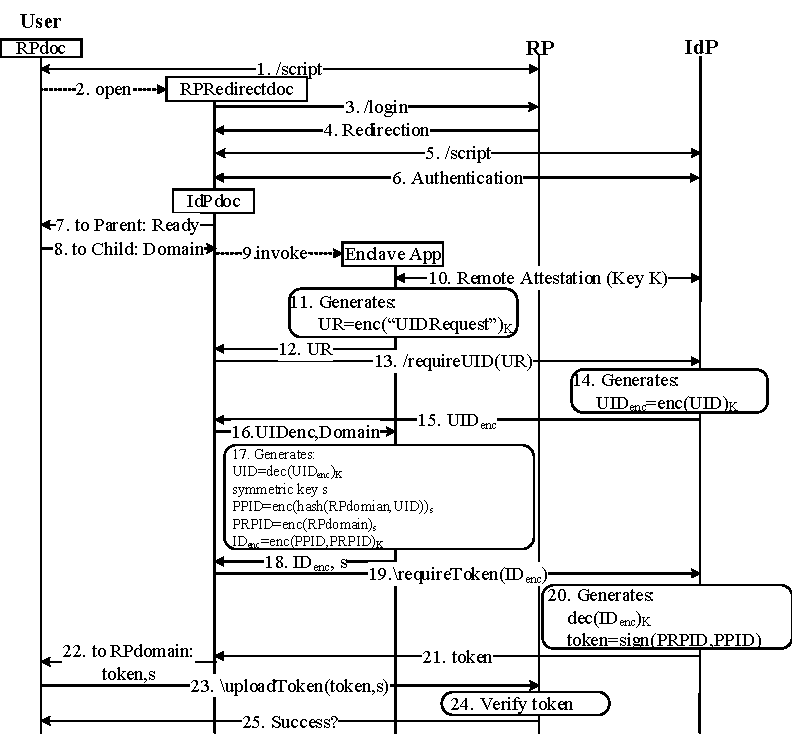
\includegraphics[width=0.8\linewidth]{fig/sgx-sso.pdf}
  \caption{The protocol flow of UP-SSO.}
  \vspace{-5mm}
  \label{fig:UP-SSO}
\end{figure*}
%The UP-SSO is compatible with OIDC, besides that the IdP service is separated into user part and server part. 
%The user agent (i.e., user-side IdP service) would obtain the UID from server part service, transform UID into the PPID, and encrypt the RPID and PPID with a one-time symmetric key to avoid IdP server digging out the RP's identity. As the enclave application is protected by SGX, it must not conduct any malicious behaviour. 
%The server-side IdP service takes the responsibility of authenticating the user, retrieving the UID for each user, and issuing the identity token (i.e., the identity proof) consisted the privacy-preserving RP and user identifier.

In this section, we will provide the detailed protocol.

%\subsection{UP-SSO procedures}
\subsection{Initialization}
%\vspace{1mm}\noindent\textbf{RP registration.} 
At the very beginning, RP needs to register its domain, RP name and other essential attributes at IdP, and obtains a signed Cert.  Thus, the  IdP can only provide the service to the qualified RP by checking the ownership of a Cert inside the enclave application.

%\vspace{1mm}\noindent\textbf{Preparation work of user .} 
Moreover, user should install the enclave application on her device before the visit targeting an RP. 

\subsection{Login Process}
Following, we provide the detailed process of each authentication flow shown as Figure~\ref{fig:UP-SSO}.
%The procedures of UP-SSO are depicted in detail in Figure~\ref{fig:UP-SSO}. 
It can be split into three phases, scripts downloading, PPIDs generation and identity proof issuing. To be noticed that, all the communication flows among user, RP server and IdP server are protected by TLS.

\vspace{0.5mm}\noindent\textbf{Scripts downloading.} This phase is for the user’s browser to download the scripts from the RP and IdP. The SSO process is started with the user's visit to an RP at her browser, and the browser downloads the RP script (step 1). Then the RP script opens a new window targeting RP login endpoint (step 2, 3). After that the user is redirected to the IdP server (step 4). Finally, the user retrieves the IdP script (step 5).

It must be noticed that, the user cannot visit IdP at step 2,3 directly. While the script in origin A opens a new window with origin B, the HTTP request to B's server will carry the key-value $Referer: A$. Thus, the RP's domain is exposed.% to IdP. 
% The scripts work as part of the user agent role.
\begin{comment}
\item[1]The SSO process is started with the user's visit to an RP at her browser, and the browser downloads the RP script. 
%The script is used to conduct the behaviour defined by RP on user side.
\item[2]The RP script opens a new window. 
\item[3]The newly opened window visits RP login endpoint.
\item[4]The user is redirected to the IdP server from RP.% login endpoint.
\item[5]The user retrieves the IdP script, which is used to deal with the interaction with other entities.% IdP server, RP script and enclave application.
\end{comment}
%It must be noticed that, the user cannot visit IdP at step 2,3 directly. While the script in origin A opens a new window with origin B, the HTTP request to B's server will carry the key-value $Referer: A$. Thus, the RP's domain is exposed.% to IdP. 
%With HTML5, a special attribute for links in HTML was introduced, that the $ref="noreferrer"$ can be used to make $Referer$ header be suppressed. However, when such a link is used to open a new window, the new window does not have a handle on the opening window (opener) anymore. The handle is necessary for UP-SSO to transmit messages between RP and IdP scripts. 
%So the redirection is adopted to avoid the HTTP header $Referer$. %and make the handle of the opening window available. 


\vspace{0.5mm}\noindent\textbf{PPIDs Generation.} In this phase, IdP script invokes the enclave application to generate the PPID. 
At first, the IdP authenticates the user (step 6). 
After that, IdP script informs RP window (step 7), and RP script sends its Cert to IdP script (step 8).  
Then IdP script asks for user's consent to visit targeting RP, and it invokes the enclave application (step 9). 
The enclave application conducts remote attestation at its initialized execution, and negotiates a symmetric key $K$ with IdP server (step 10).
Following the enclave application generates the UID request by encrypting request information with $K$ (step 11). 
The request is sent to IdP script (step 12) and transmitted to IdP server (step 13). 
IdP encrypts $UID$ with $K$ (step 14), and transmits it to enclave application through IdP script (step 15, 16).  
While receiving the encrypted $UID$, the enclave application derives the $UID$, verifies the Cert and achieves RP's domain from it, generates the symmetric key $S$, encrypts the RP's domain as the  $PPID_{RP}$, encrypts the hash of RP's domain and UID as the $PPID_U$, and encrypts $PPID_{RP}$ and $PPID_U$ with $K$ (step 17). 
Finally the encrypted IDs and $S$ are sent to IdP script (step 18). 

The $PPID_U$ must be the encrypted hash of RP's domain and UID, instead of the plain digest. It avoids the IdP to find out multiple logins targeting the same RP or not, as the hash of same RP's domain would be always the same. 

%Moreover, there are some types of parameters required in OIDC protocol to be carried in the SSO request, such as $response\_type$ and $scope$. In this paper, we would not mention these attributes, and only focus on the necessary parameters. 
\begin{comment}
\item[6]At first, the IdP authenticates the user.
\item[7]After the IdP script is downloaded, it sends the ready signal to its opener (i.e., the RP window).
\item[8]RP script sends the RP's Cert back to IdP script. 
\item[9] The IdP script shows RP name to user to make sure user would not visit malicious RP, and then it invokes the enclave application.
\item[10]The enclave application conducts remote attestation at its initialized execution. After the remote attestation, enclave application and IdP server share a symmetric key $K$.
\item[11]The enclave application generates the UID request (i.e., $UR$) by encrypting request information with $K$.
\item[12]$UR$ is sent to IdP script.
\item[13]Then the user starts the UID request to IdP.
\item[14]IdP encrypts $UID$ with $K$.
\item[15]IdP script receives encrypted $UID$ from IdP.
\item[16]IdP script transmits encrypted $UID$ and RP's domain to enclave application.
\item[17]The enclave application derives the $UID$ with $K$, verifies the Cert, achieves RP's domain from Cert, generates the symmetric key $s$, encrypts the RP's domain with key $s$ as the transformed RP ID (i.e., $PRPID$), encrypts the hash of RP's domain and UID as the $PPID$, and encrypts $PRPID$ and $PPID$ with $K$.
\item[18]Enclave application sends the encrypted IDs and $s$ to IdP script. 
\end{comment} 
%The PPID must be the encrypted hash of RP's domain and UID, instead of the plain digest. It avoids the IdP to find out multiple logins targeting the same RP or not, as the hash of same RP's domain would be always the same. 

%Moreover, there are some types of parameters required in OIDC protocol to be carried in the SSO request, such as $response\_type$ and $scope$. In this paper, we would not mention these attributes, and only focus on the necessary parameters. 

\vspace{0.5mm}\noindent\textbf{Identity proof issuing.} In this phase, IdP issues an identity proof containing the encrypted $PPID_{RP}$ and $PPID_U$. And the RP verifies the token.
At the beginning user sends the encrypted $PPID_{RP}$ and $PPID_U$ to IdP for identity proof (step 19). 
Then the IdP server derives the $PPID_{RP}$ and $PPID_U$, signs the $Token$ consisted of $PPID_{RP}$ and $PPID_U$ as the identity proof (step 20), and sends it to IdP script (step 21). 
The IdP script then sends the $token$ and $s$ to the origin RP's $Domain$ through $postMessage$ (step 22), and  RP script uploads them to RP server (step 23). 
The RP server verifies the signature with IdP's public key, compares the $PPID_{RP}$ carried with identity proof with self-generated one, and derives the constant user account from $PPID_U$ (step 24). 
%generates the $PRPID$ with its domain and key $s$, and compared it with the one carried by $token$. If the two $PRPID$s are equaled, RP decrypts the user's account from $PPID$, and finds out the related user information in its database (step 24). 
At the end, RP returns the login result back to user (step 25).


\begin{comment}
\item[19]User sends the encrypted $PRPID$ and $PPID$ to IdP for identity proof.
\item[20]The IdP server derives the $PRPID$ and $PPID$, signs the $token$ consisted of $PRPID$ and $PPID$ as the identity proof.
\item[21]IdP sends identity token to enclave application.
\item[22]The IdP script then sends the $token$ and $s$ to the origin RP's $Domain$ through $postMessage$.
\item[23]The RP script uploads the $token$ and key $s$ to RP server.
\item[24]The RP server firstly verifies the signature with IdP's public key, then generates the $PRPID$ with its domain and key $s$, and compared it with the one carried by $token$. If the two $PRPID$s are equaled, RP decrypts the user's account from $PPID$, and finds out the related user information in its database.
\item[25]RP returns the login result back to user.
\end{comment} 

%The origin in step 22 is essential for secure identity token transmitting.
%It guarantees that only the script running in the RP window can receive the $token$, that avoids the man-in-the-middle attack.

